\chapter*{Force from Bone conductor to the skull}
To ensure that the \gls{bc} does not excite the comfortable force to the skull, a force test of the \gls{bc} against the head was made. To measure the force from the \gls{bc} a force measuring system was developed and placed at the ear position of the B\&K Head and Torso simulator 4128.    

\section*{Materials and setup}
To measure the force of the \gls{bc} on the skull, the following materials are used:


\begin{table}[H]
\centering
\caption{Equipment list}
\label{equip_list}
\begin{tabular}{l|l|l|l l}
Description         & Model                                                      & Serial-no  & AAU-no \\ \hline
Processor         & Arduino UNO                                              & 170294662  & -  \\
strain gauge amplifier     & Analog Devices Eval-cn0216                              & 706609 1631   & - \\
strain gauge     & -                             & -   & - \\
Weight     & KERN EMB 500-I GN                             & -   & - \\
Bold and washers    & -                            & -   & - \\
Head and torso simulator     & B\&K Type 4128                              & 08453-00   & 1407972 \\
Analysis software   & MATLAB \textsuperscript{\textregistered} R2018b & -          & -     
\end{tabular}
\end{table}

\begin{figure}[H]
\centering
\def\svgwidth{\columnwidth}
\input{figures/appendix/force_meas.pdf_t}
%\input{figures/appendix/guitar_frequency_test.pdf_tex}
\caption{Setup for force measurement.}
		\label{fig:appendix:force_meas_system}
\end{figure}

\section*{Calibration procedure}
To perform the force measurement, a evaluation code example for the Analog devices EVAL-CN0216-ARDZ was loaded intro the Arduino due. The code write a digital number to the serial bus which correspond to a weight. For correspond a digital number to a given weight, the system have to be calibrated. A calibration is done as following: 

\begin{enumerate}
\item The materials are set up as in \autoref{fig:appendix:force_meas_system}.
\item A serial read is set up in MATLAB
\item The strain gauge was placed in water level \autoref{fig:strain_gauge_water}.
\item  Five weight combination of bold and washers was chosen.
\item  For every chosen combination, the weight of the bold and washers was measured.
\item For every chosen combination, the weight of the bold was placed on the strain gauge and the digital number was measured, see \autoref{fig:strain_gauge_weight}. 
\item For every chosen combination, the measurement was done over \SI{30}{second} and the mean was calculated. The corresponding number to weight is in \autoref{apend:cal_result}
\end{enumerate}

\begin{figure}[H]
\centering
\begin{subfigure}[htbp]{0.45\textwidth}
		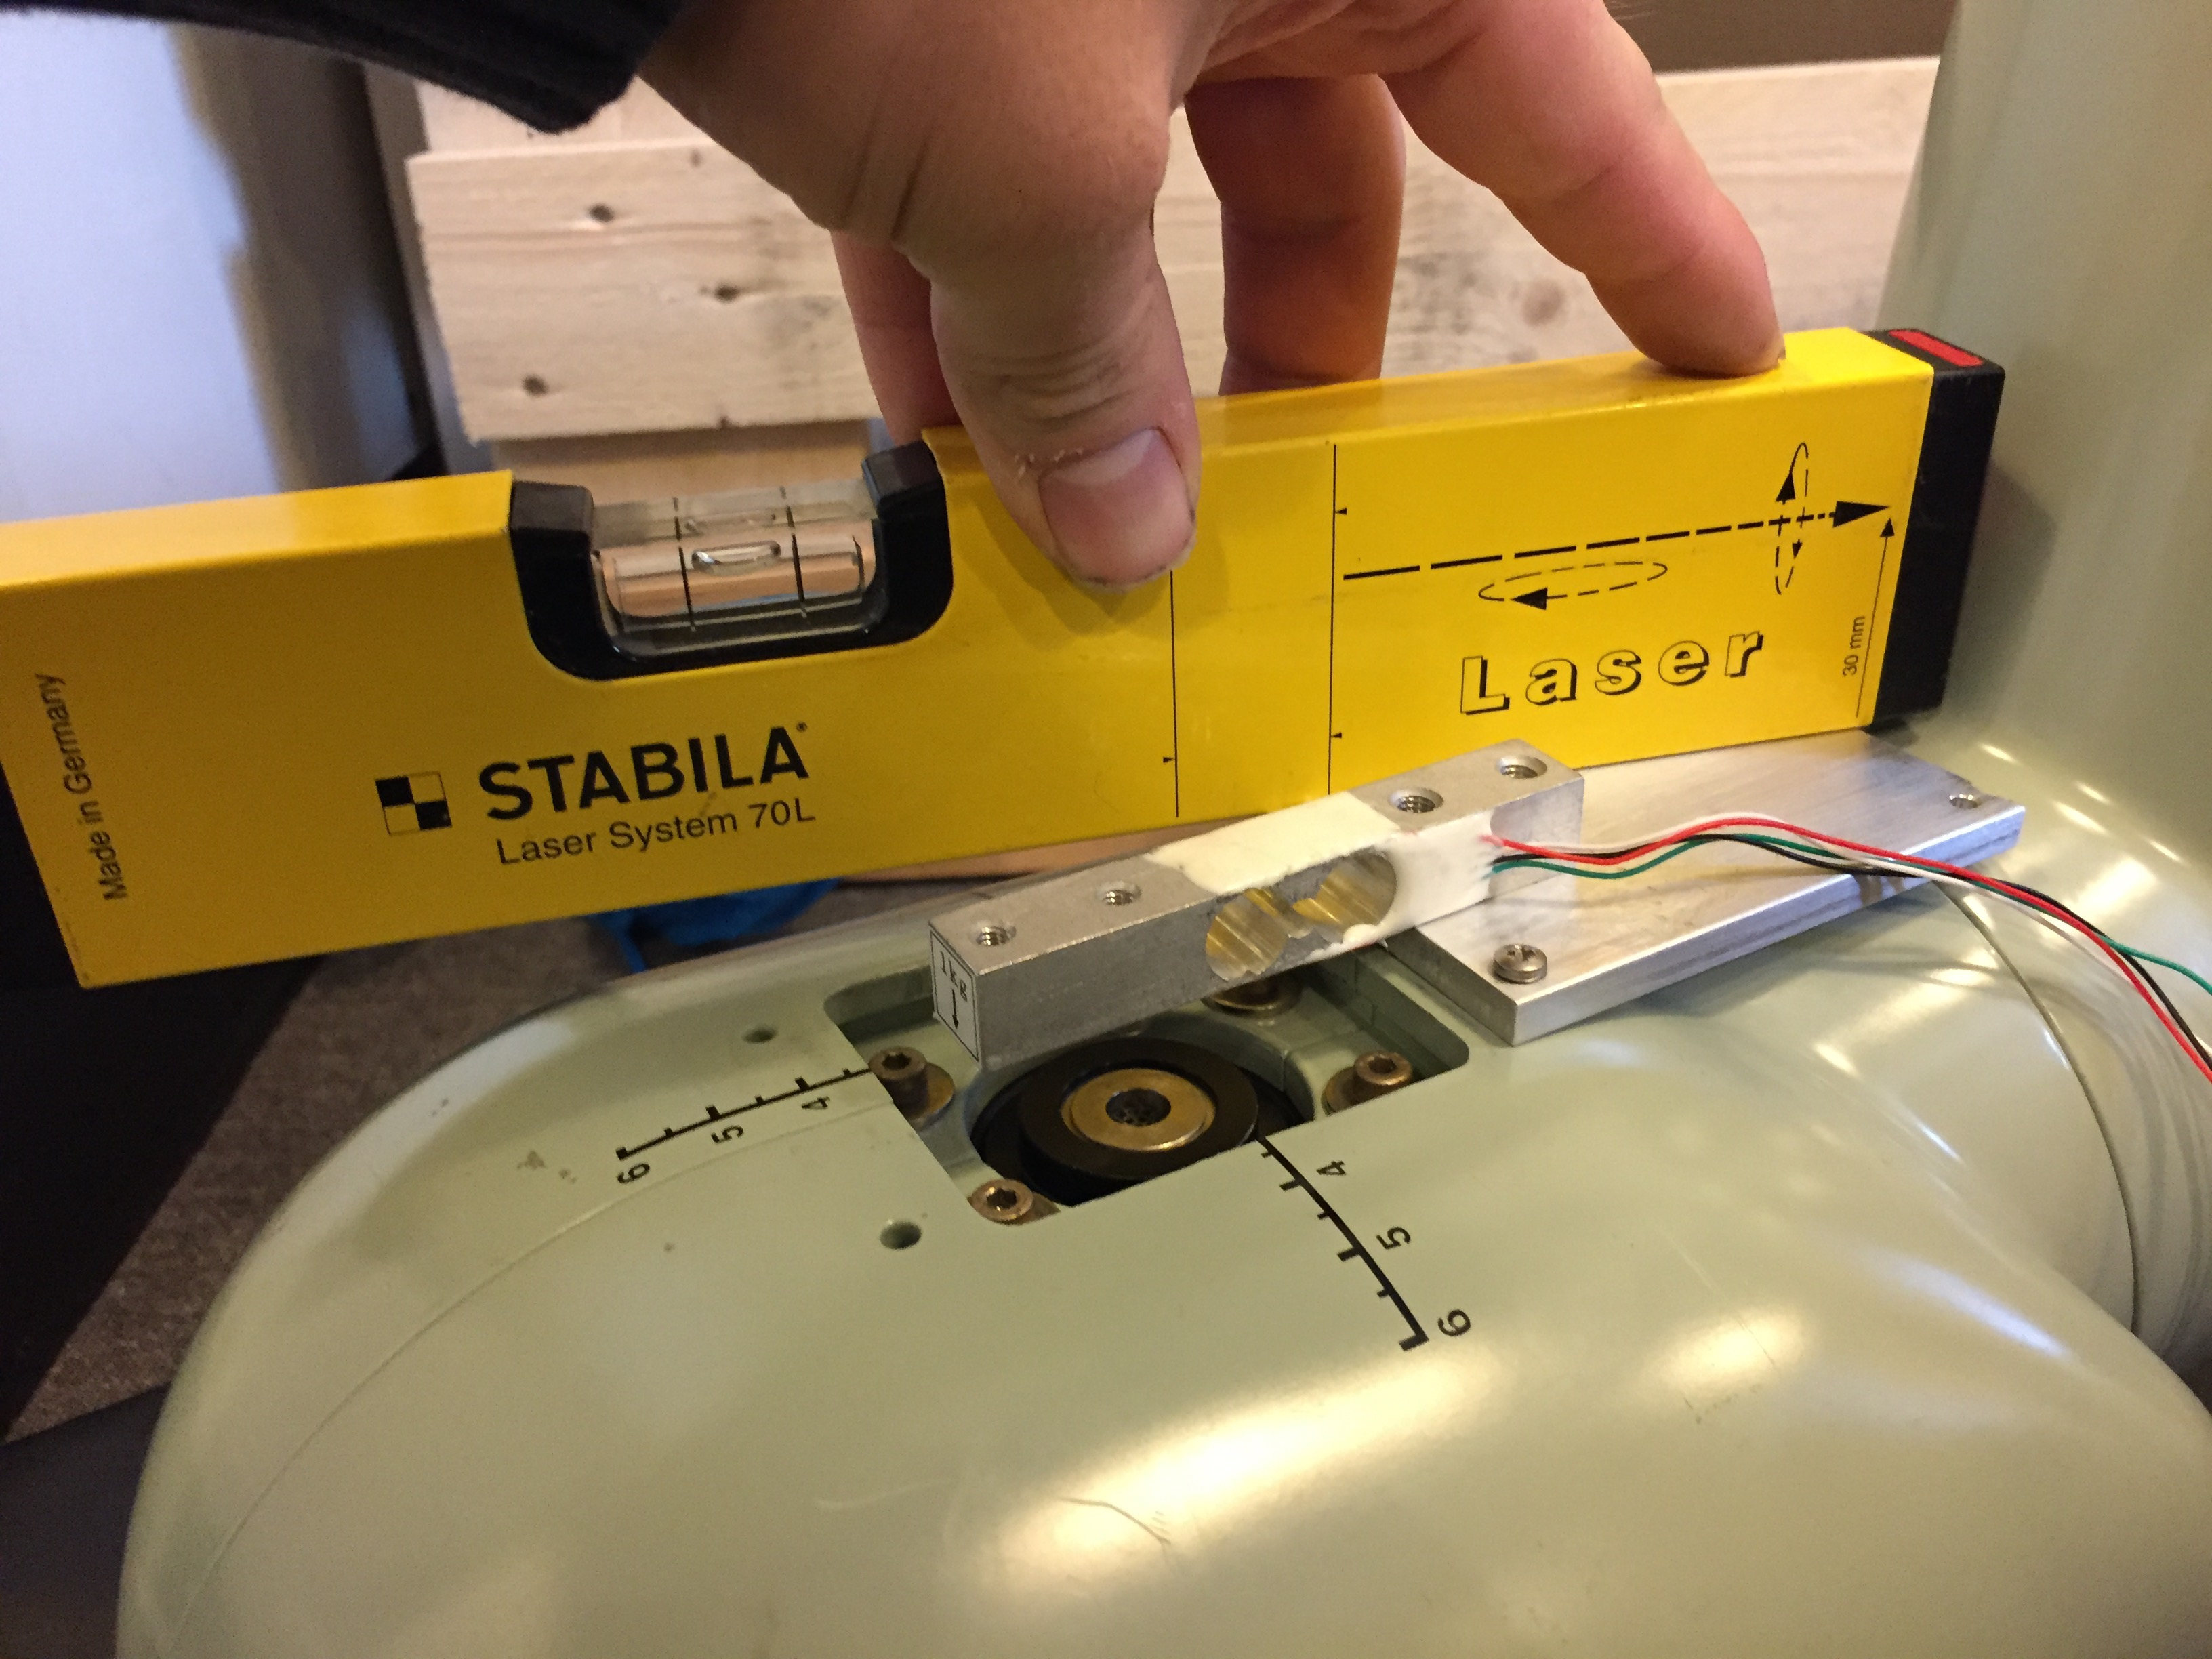
\includegraphics[width=1\textwidth]{IMG_0864}
		\caption{The water level check position of the strain gauge}
		\label{fig:strain_gauge_water}
\end{subfigure}\vspace{10pt}
\begin{subfigure}[htbp]{0.45\textwidth}
		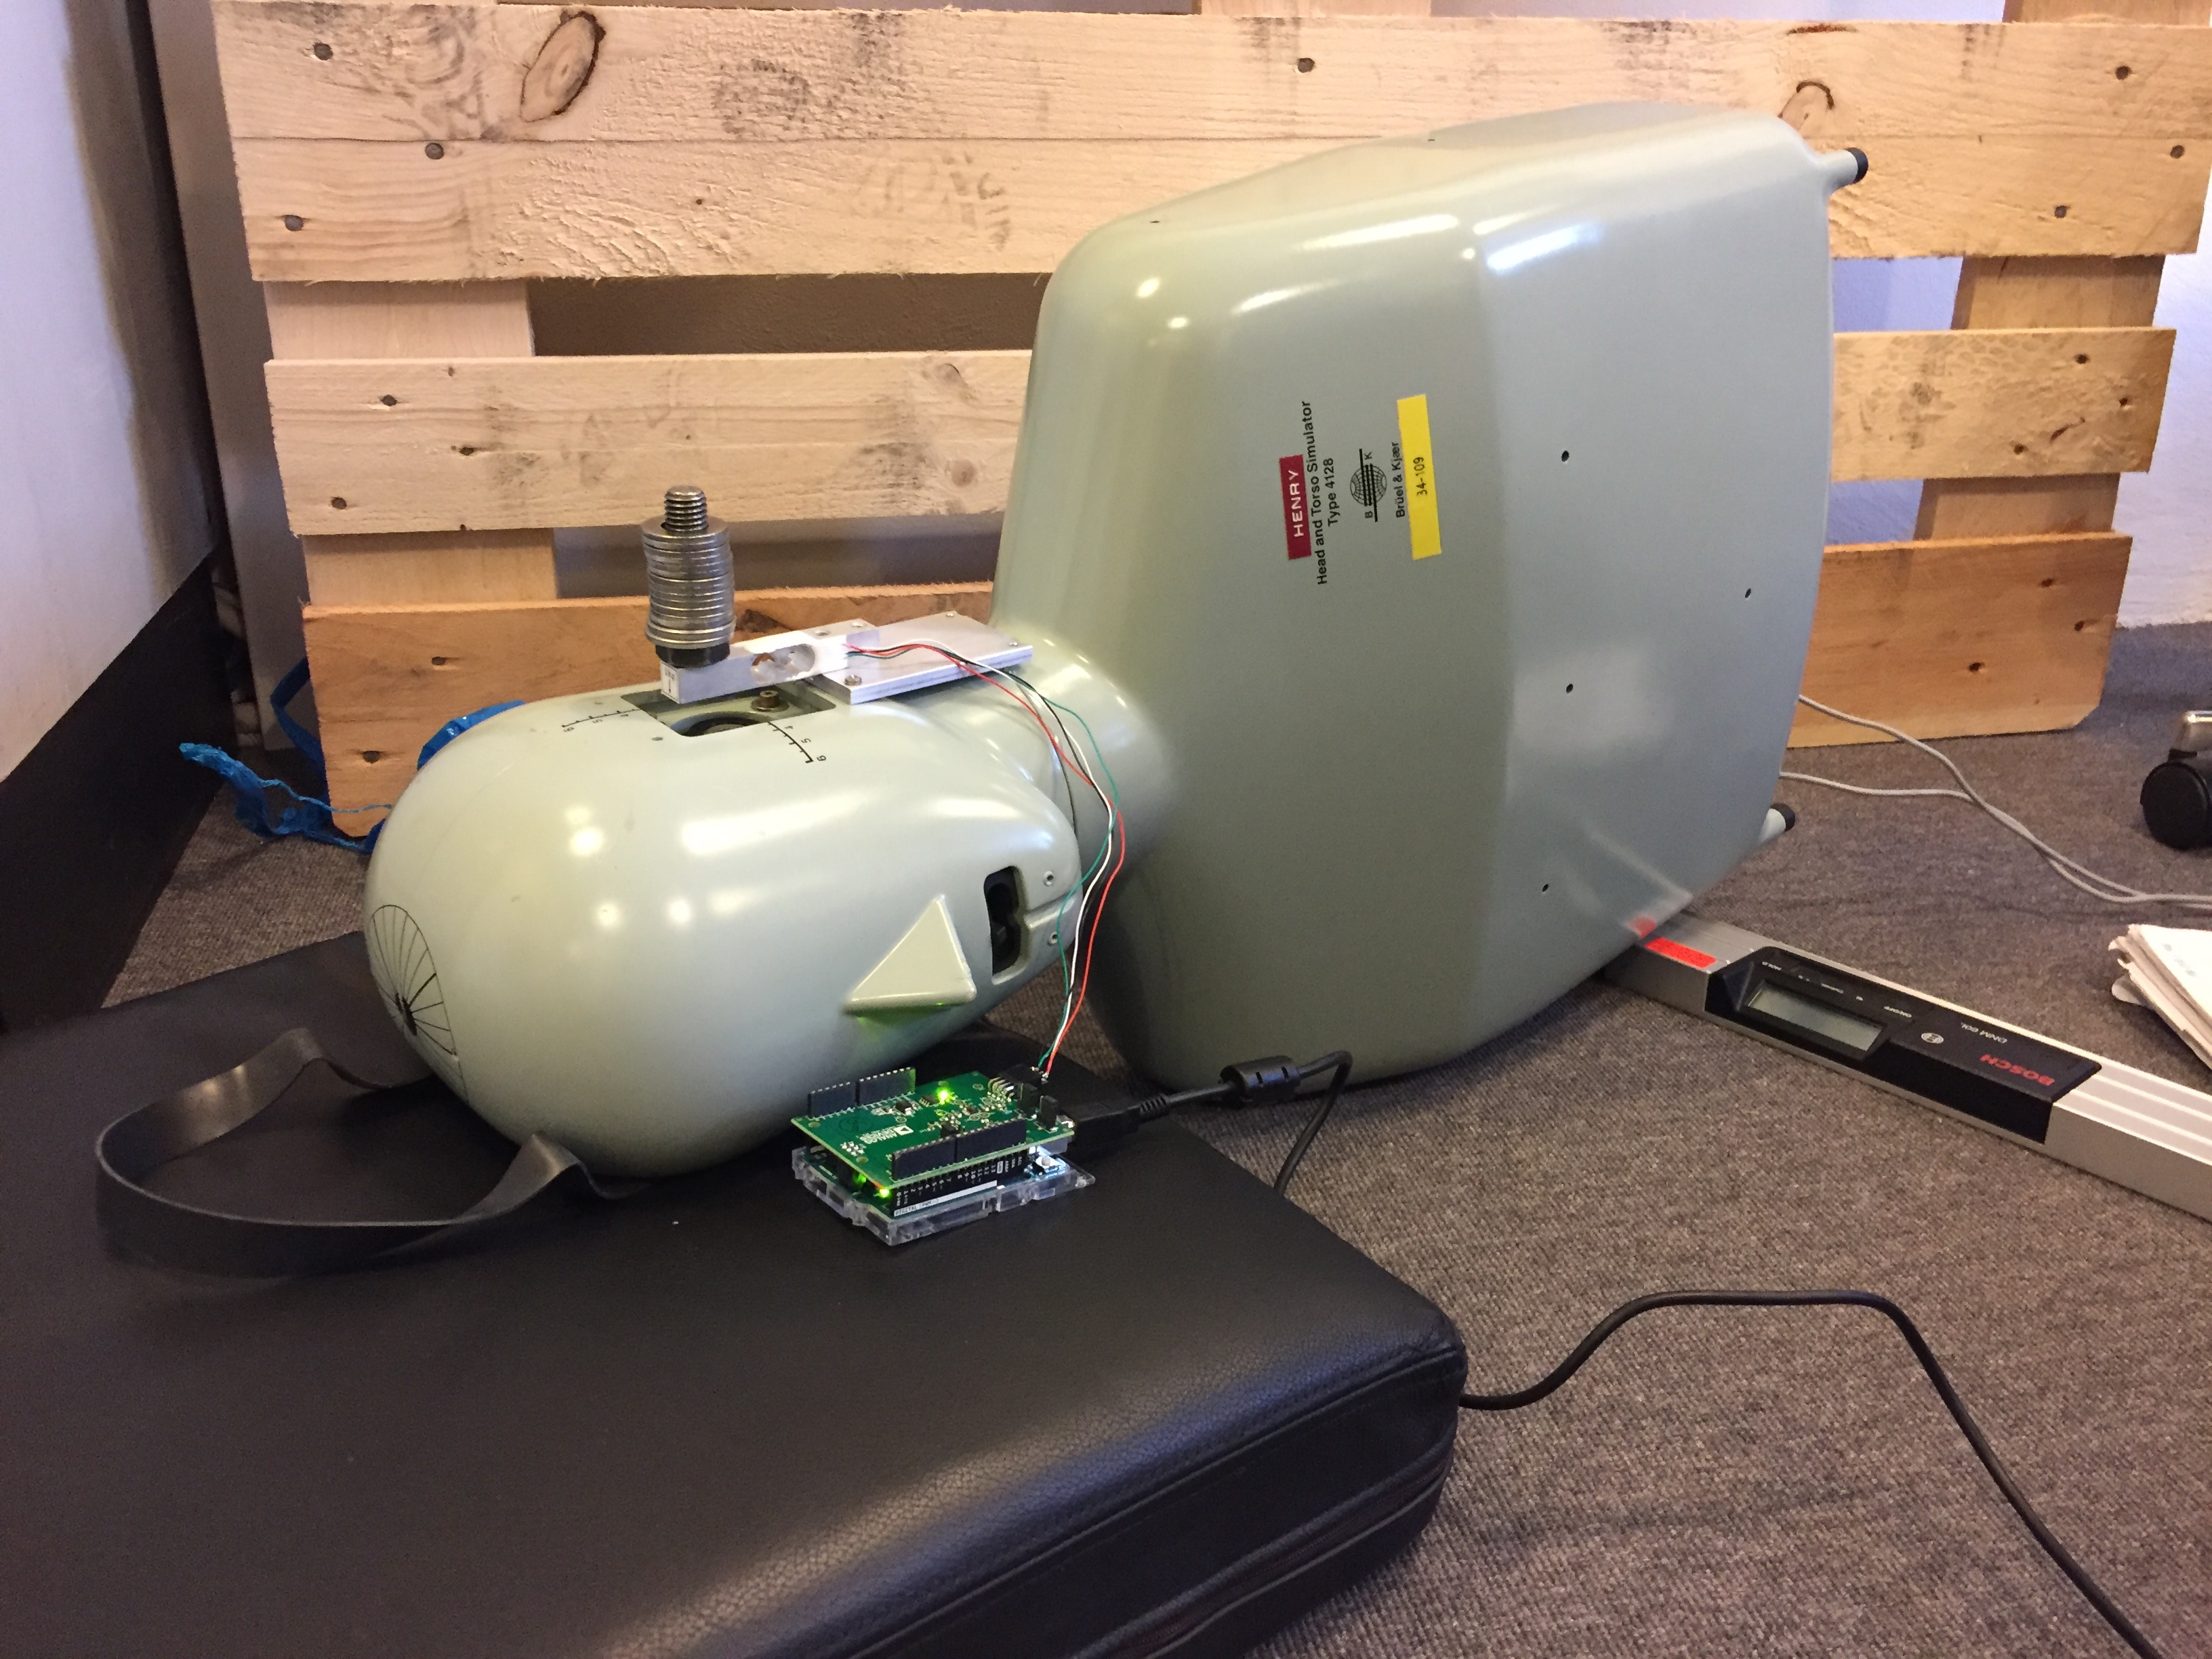
\includegraphics[width=1\textwidth]{IMG_0865}
		\caption{The position of the weight on the strain gauge}
		\label{fig:strain_gauge_weight}
\end{subfigure} \hspace{10pt}
\caption{The placement of the weight for calibration}
\label{fig:bc_holder}
\end{figure}


The following \autoref{code:serial_read_ard_init} is used for setting up the serial read in MATLAB.

\includeCode{serial_read_ard.m}{matlab}{11}{13}{Serial read setup}{code:serial_read_ard_init}{./code/weight_measurement/}

The following \autoref{code:serial_read_ard} is used for serial read in MATLAB.

\includeCode{serial_read_ard.m}{matlab}{19}{27}{Serial read setup}{code:serial_read_ard}{./code/weight_measurement/}

The result is as following \autoref{apend:cal_result}

\begin{table}[H]
\centering
\caption{The mean read out of a specified weight}
\label{apend:cal_result}
\begin{tabular}{l|l}
Weight \si{\gram} & Arduino read out \\ \hline
75.3              & 8678100          \\
118.0             & 8805000          \\
156.4             & 8919100          \\
194.1             & 9031200          \\
226.7             & 9127800         
\end{tabular}
\end{table}

The calibration point in \autoref{apend:cal_result} is used in the MATLAB function \texttt{polyfit} with linear least square fitting. The output is two coefficient which can be used in the MATLAB function \texttt{polyval} along with the read out for the weight measurement. 


\section*{Test procedure}


\begin{enumerate}
\item The materials are set up as in \autoref{fig:appendix:force_meas_system}.
\item The hair band is putted on the head of the B\&k type 4128 with the \gls{bc} such that the \gls{bc} press on the strain gauge, see \autoref{fig:bc_hair_band}
\item The force is calculated.
\item The hair band and \gls{bc} is removed form the head and putted on again
\item Do force measurement
\item  Repeat ten times and calculate the mean.
\item  The test is repeated with the original \gls{bc} metal holder, see \autoref{fig:bc_metal_holder}.
\end{enumerate}



\begin{figure}[H]
\centering
\begin{subfigure}[htbp]{0.33\textwidth}
		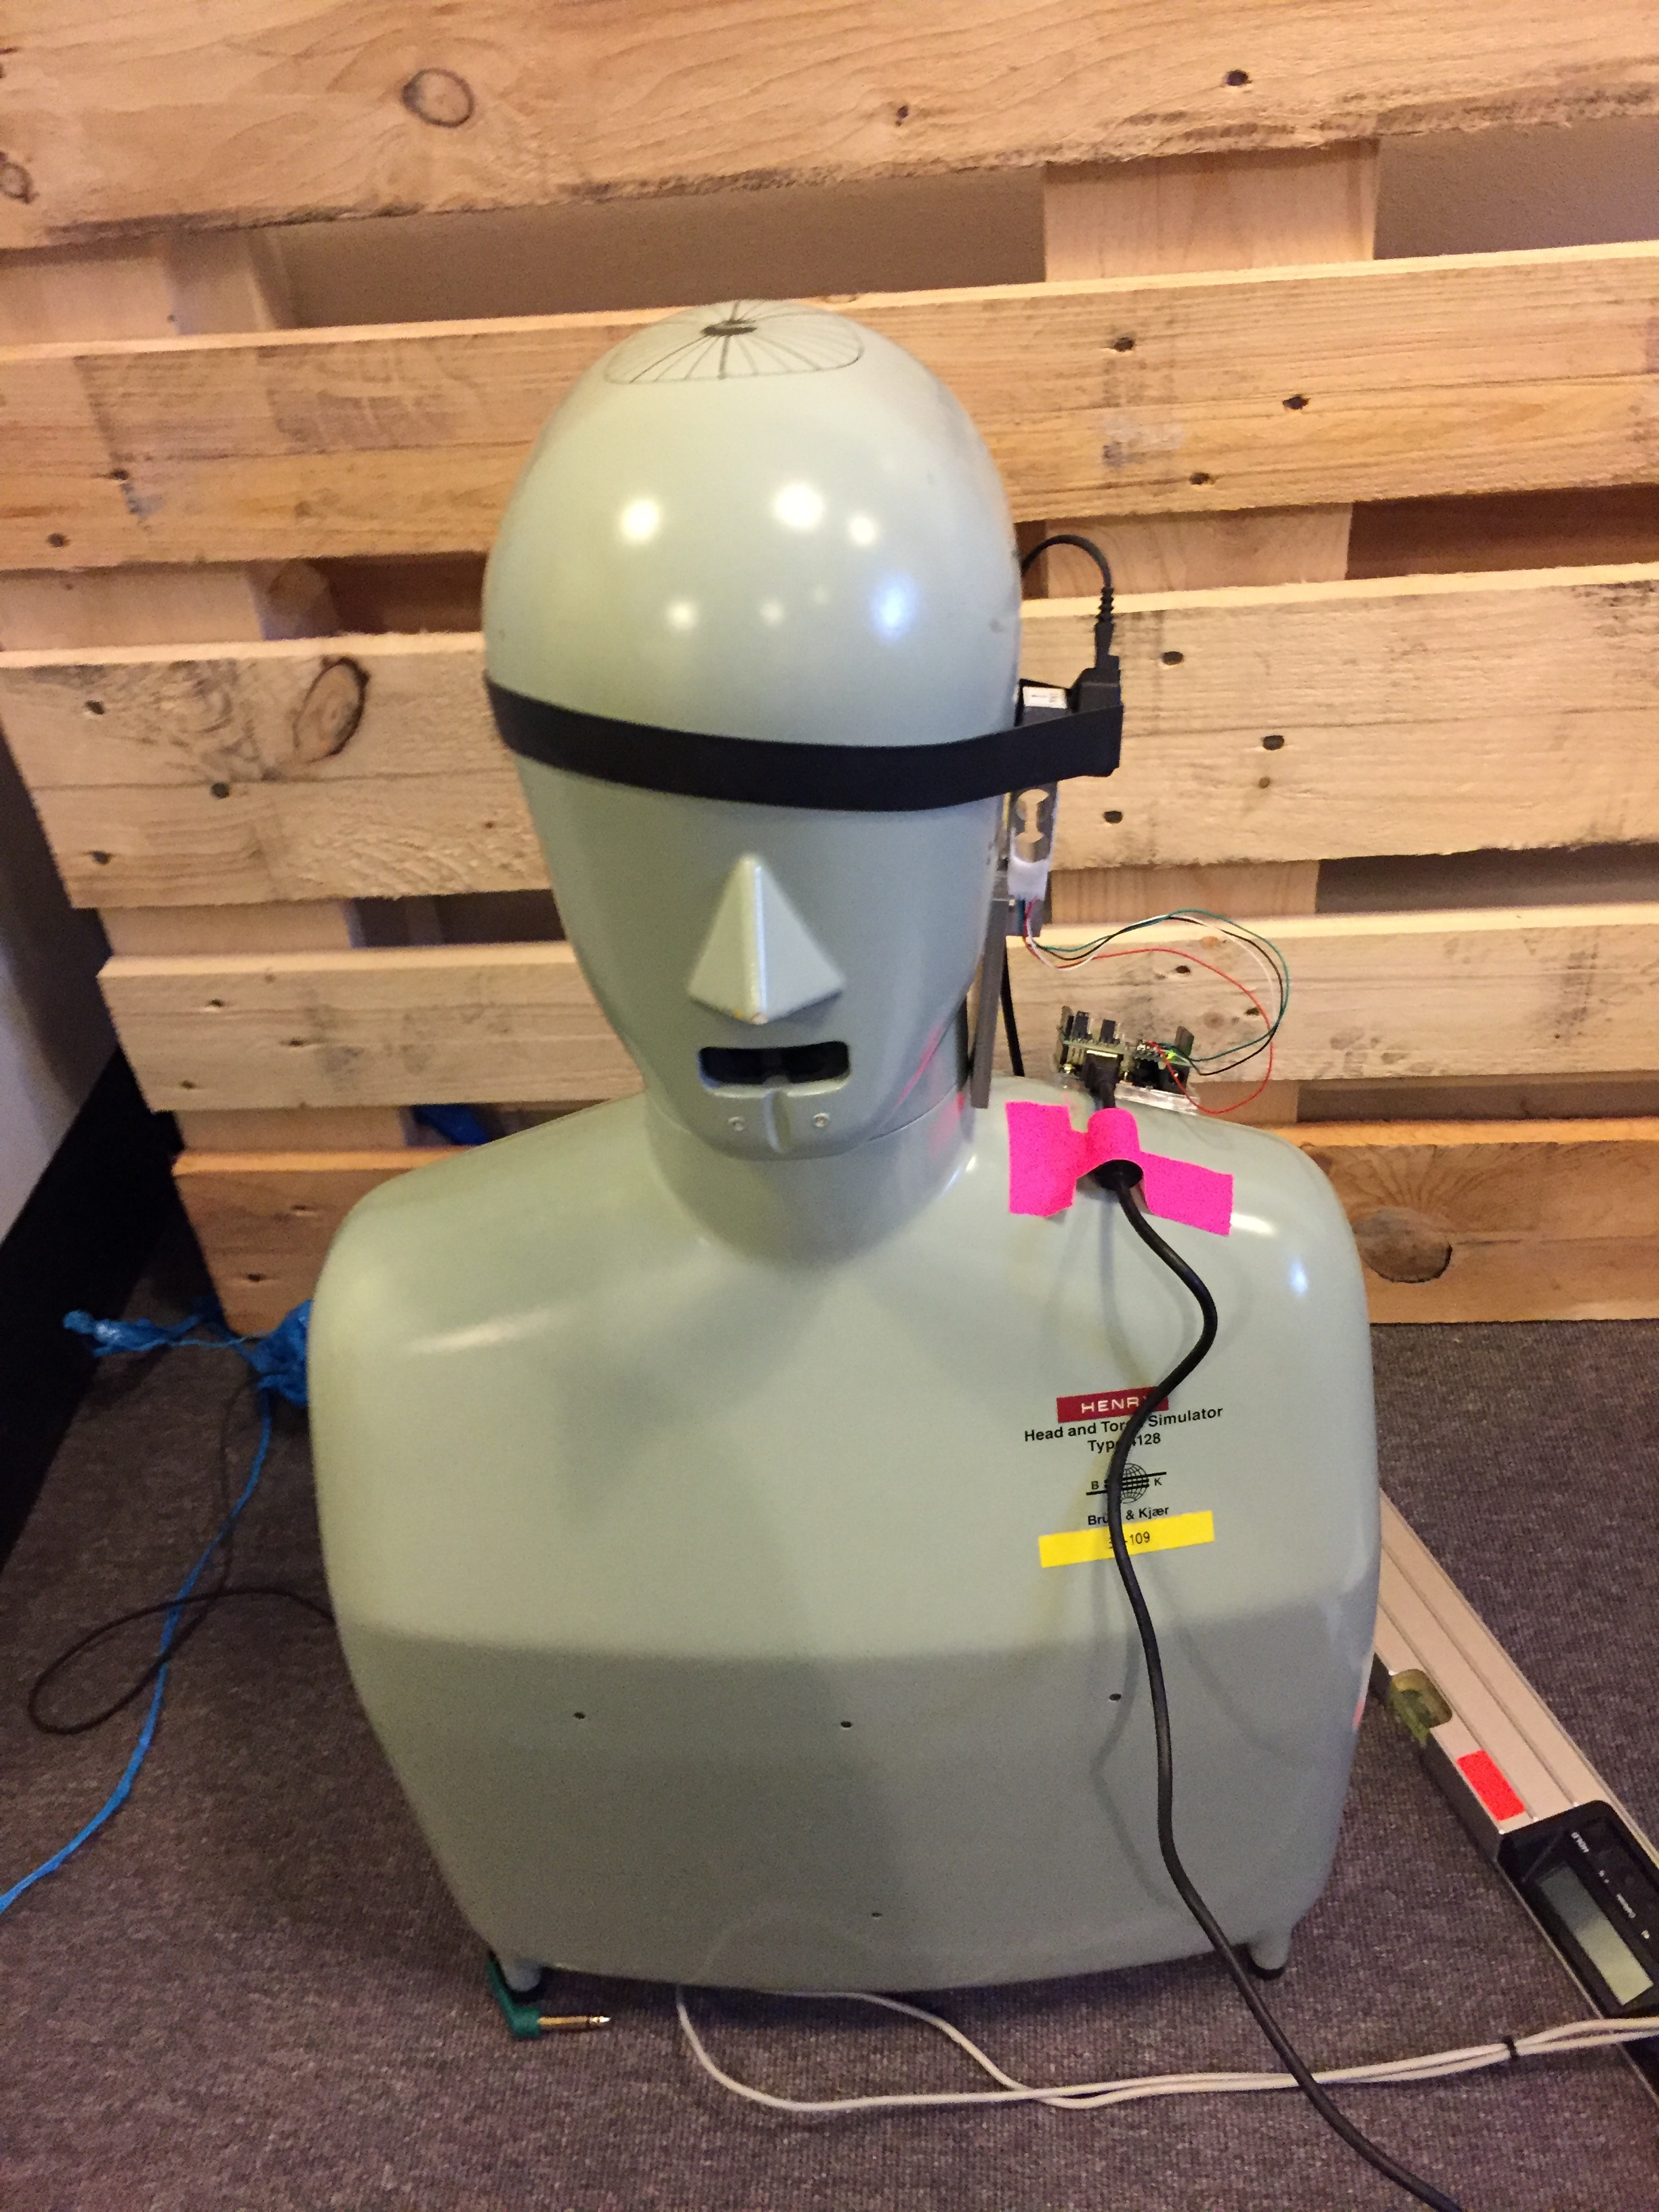
\includegraphics[width=1\textwidth]{IMG_0871}
		\caption{The position of the \gls{bc} with hair band}
		\label{fig:bc_hair_band}
\end{subfigure}\vspace{10pt}
\begin{subfigure}[htbp]{0.60\textwidth}
		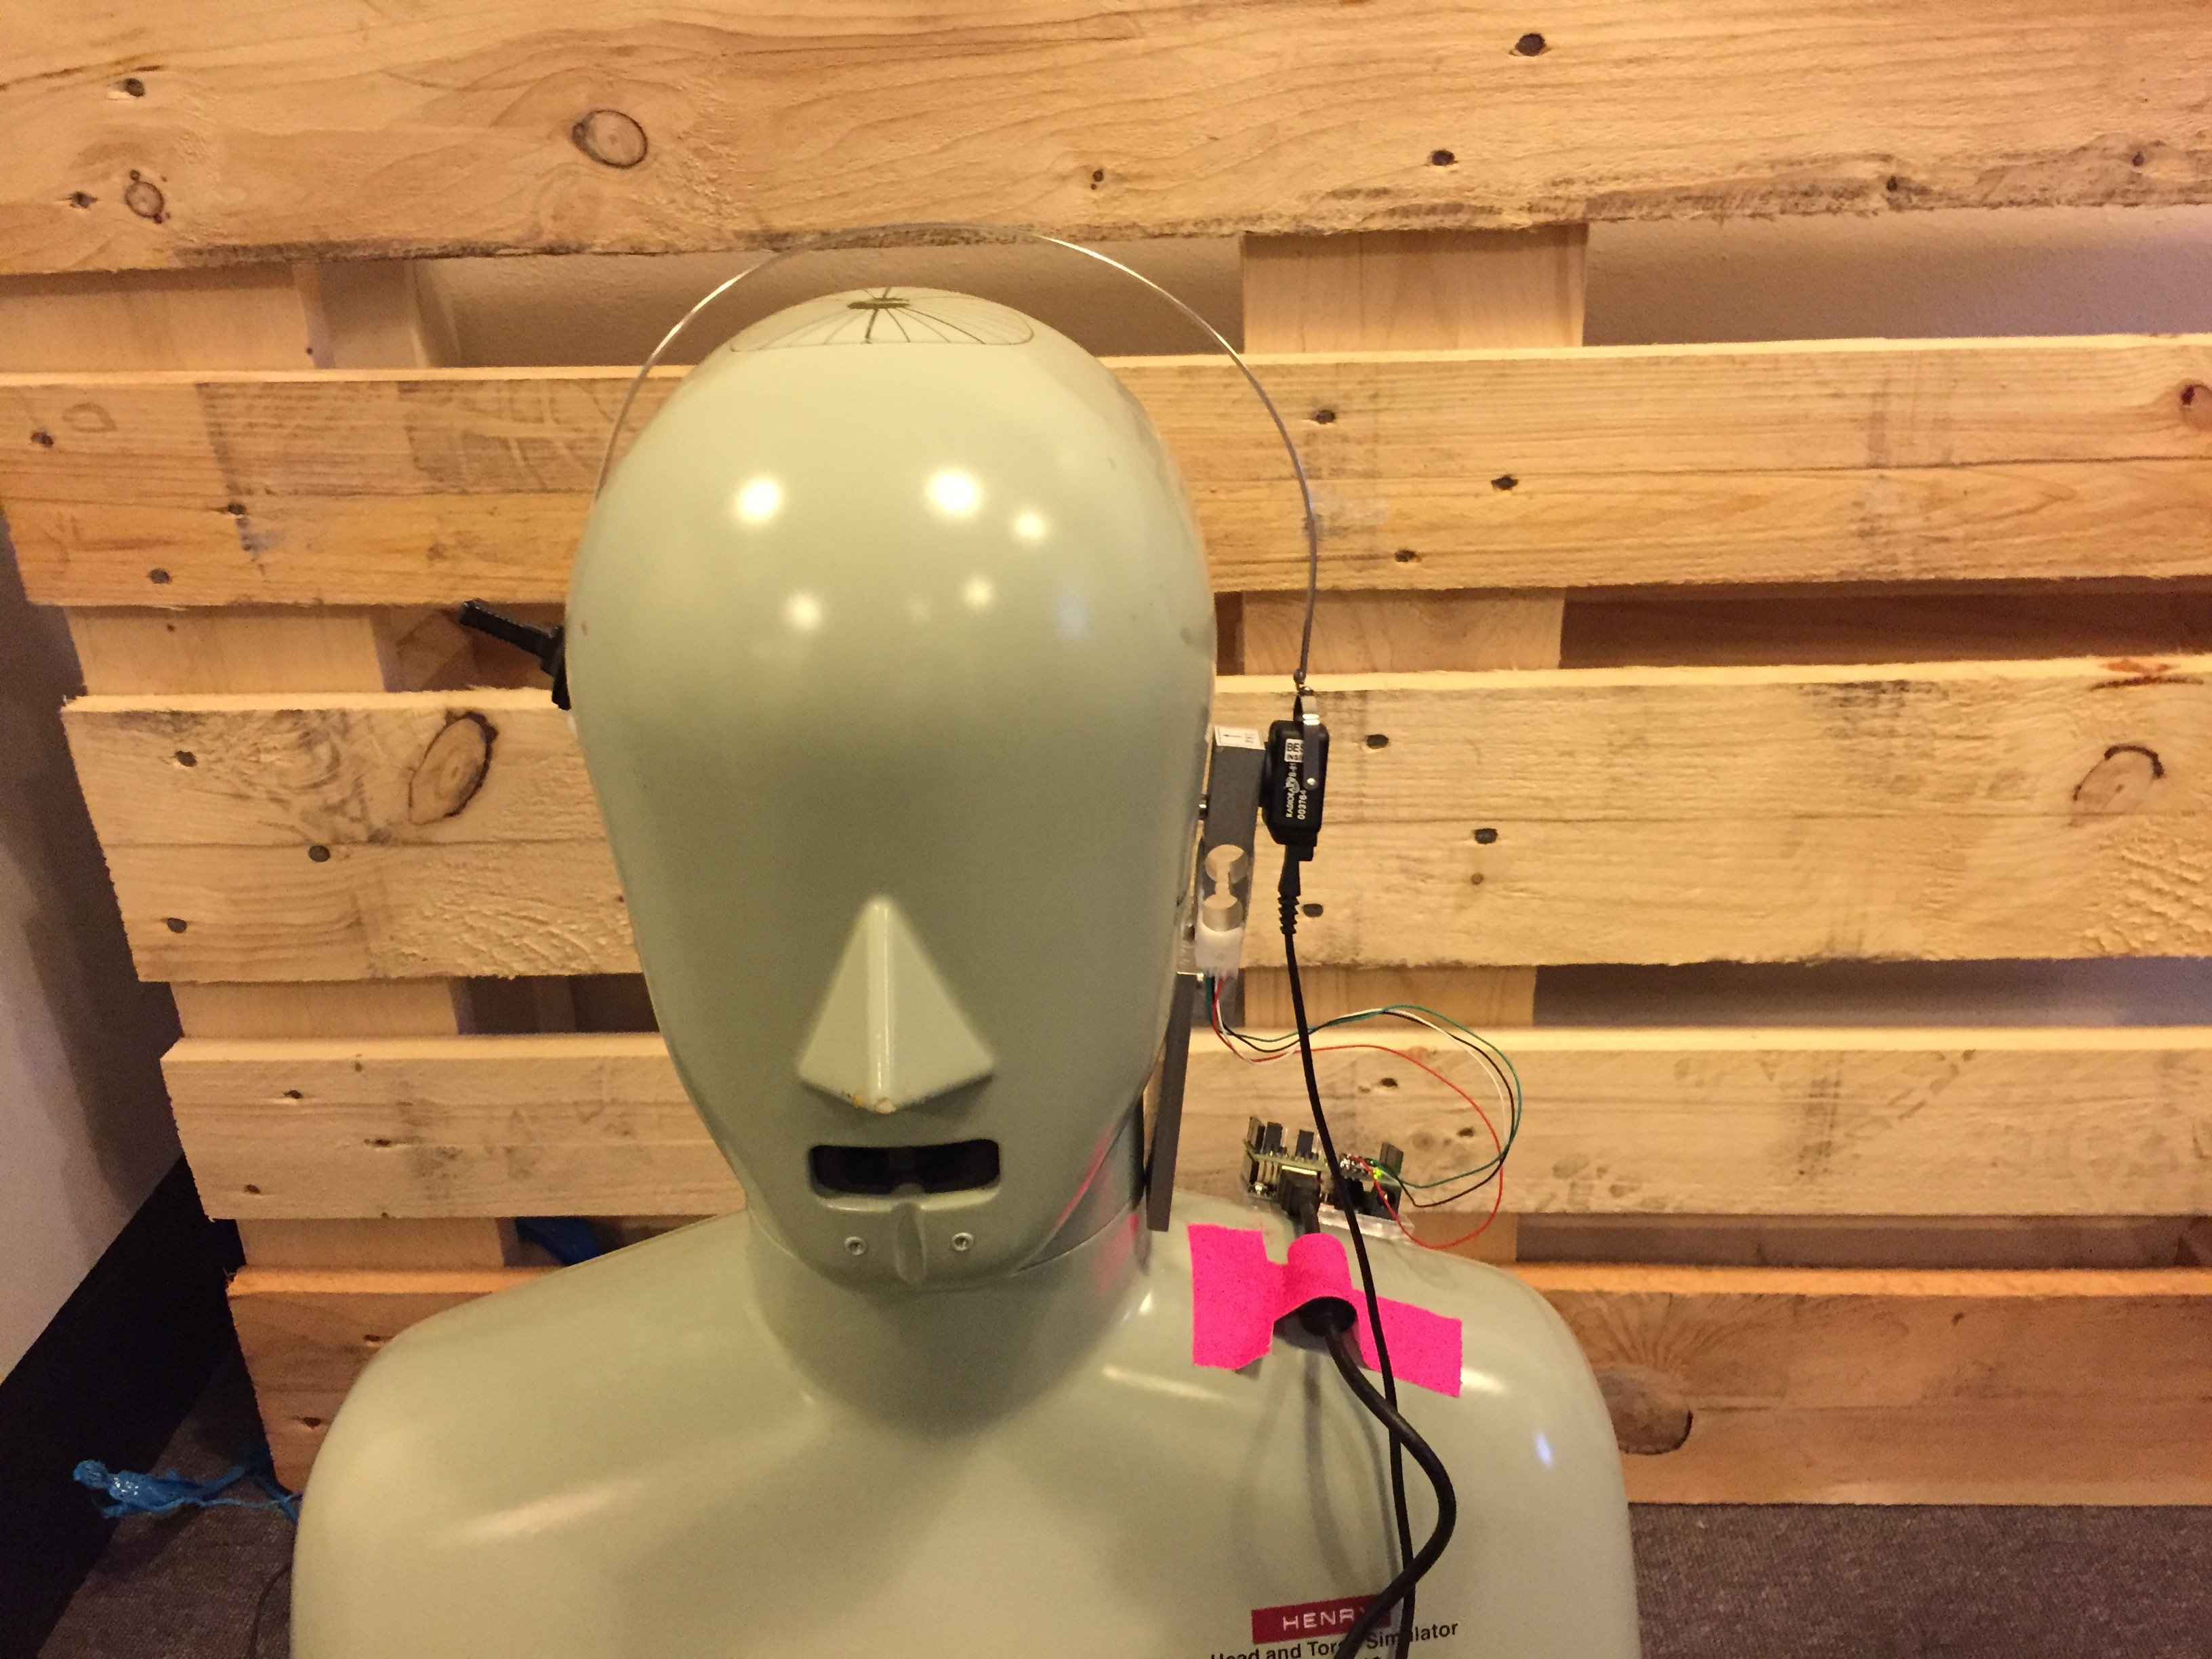
\includegraphics[width=1\textwidth]{IMG_0874}
		\caption{The position of the \gls{bc} with the original metal bolder for Radioear B81}
		\label{fig:bc_metal_holder}
\end{subfigure} \hspace{10pt}
\caption{The placement of the \gls{bc} for force test}
\label{fig:bc_holder}
\end{figure}


The following \autoref{code:serial_read_ard_cal} is used for reading the read out and calculate the force in MATLAB.

\includeCode{serial_read_ard.m}{matlab}{98}{107}{Force measurement}{code:serial_read_ard_cal}{./code/weight_measurement/}


\section*{Results}


\begin{table}[H]
\centering
\caption{The measurement result with both the original holder and the rubber band holder}
\label{apend:weight_result}
\begin{tabular}{ll}
Force with original metal holder [\si{newton}] & Force with the rubber hair band [\si{newton}] \\
7.49                                           & 4.10                                          \\
7.34                                           & 4.00                                          \\
7.57                                           & 4.40                                          \\
7.77                                           & 3.89                                          \\
7.47                                           & 4.09                                          \\
7.63                                           & 4.83                                          \\
7.47                                           & 4.09                                          \\
7.30                                           & 4.77                                          \\
7.33                                           & 3.37                                          \\
7.57                                           & 4.73                                         
\end{tabular}
\end{table}

The mean force with the rubber band is \SI{4.23}{\newton} and the mean force with the original holder is \SI{7.49}{\newton}. The standard diviation of the rubber band is \SI{0.46}{\newton} where the standard diviation of the original holder is \SI{0.15}{\newton} 


